%
% MpLtX --- a LaTeX Template for Modern Physics Lab
% Copyright (C) 2013 Modern Phys. Lab, School of Phys., Peking Univ.
%
%   MpLtX is a template for experiment report of Modern Physics Lab in
% Peking University. This template depends on the "revtex4.1" package from
% APS Journals <http://publish.aps.org/revtex/revtex-faq>
%
% To use this template, you should open the package download from APS Journals'
% website as above and follow instructions from the README file in the package.
%
% LaTeX is marvelous for math formulae composition. However, the script grammar
% is rather difficult to handle. Maybe at the beginning, it's convenient to
% generate a pretty document. The deeper you went, more weird grammar you got.
% Before you found out the whole fantesy-like world built by Knuth, Lamport and
% numerous contributors, you would get numerous strange errors unclearly
% reported by compiler.
%
% Anyway, a lot of people wish to find a general document system which is both
% easy to use and strong enough to conveniently DIY. Word is easy to use.
% However, Word can not produce perfect document in art --- the position and
% size are not well calculated. By the way, it's such a pain to do simple but
% repeating work in Word such as formating title, generate large data table
% and etc. These works can be easily done in LaTeX if you know a little about
% programming. HTML is a easy-to-use language to create static document. It is
% compatible on all the machines currently because all you need is a simple
% browser (Firefox, Chrome or IE). In HTML5, the latest version of HTML, you
% can do colorful presentation about the report. You can present dynamic
% figures to present your idea clearly. However, the biggest problem for HTML
% is that this never renders a beautiful math formula in a simple way. HTML
% indeed has a math engine named as MathML. But this guy is notorious for its
% unreadable script grammar. So HTML+TeX --- the project MathJax, becomes a
% candidate of our dream communication media or e-document form. However, it is
% still under development. If you are interested in Java, JLaTeXMath package may
% be also a proper one since it provides a LaTeX renderer in Java.
%
% This template is modified by students in Peking University.
%   I am Sun Sibai. Cao Chuanwu shared the draft on RenRen Network. However,
% the draft did not match the requirement at all. It seems that Cao Chuanwu
% did not modified the style from package. He just put the origin content
% into LaTeX format.
%   I changed the style to satisfy the format requirement and fixed some problem
% about the incompatibility within the packages.
%
% So, if you have suggestions, please improve this template with your power. We
% will be always glad to see our work useful, popular and wonderful!
%
% This template has been tested in TeXLive 2012 with the command:
% $ xelatex mpltx.tex
% compile twice.
%
% Anyone can modify this template, but don't forget to list the previous
% developers and add yourself in.
%
% Sun Sibai <niasw@pku.edu.cn>
% Cao Chuanwu <>
%
\RequirePackage{fixltx2e} %This package in CTeX is not compatible with revtex4-1
\documentclass[aps,pre,12pt,preprint,onecolumn,showpacs,showkeys]{revtex4-1}
\usepackage{ctex}
\usepackage{setspace,dcolumn}
\usepackage{subfig}
\usepackage{hyperref}
\usepackage{graphicx,psfrag,epsfig}
\usepackage[font=small,format=plain,labelfont=bf,textfont=it,justification=raggedright,singlelinecheck=false]{caption}
\usepackage{amsmath,amsfonts,amssymb,amsthm,bm,upgreek}
\usepackage{geometry}
\usepackage[mathscr]{eucal}
\usepackage{siunitx}
\usepackage{booktabs}

%\usepackage{background} %Waterstamp package
%\SetBgContents{...的实验报告} %Waterstamp to prevent copying
%\SetBgScale{5} %Waterstamp setting
\hypersetup{colorlinks=true}
\geometry{top=2.54cm,bottom=2.54cm,left=3cm,right=3cm}
\renewcommand\appendixname{附录}
\renewcommand\abstractname{摘要}
\renewcommand\tablename{表}
\renewcommand\figurename{图}
\makeatletter
\def\@pacs@name{\songti\zihao{-4}{\bf PACS码:}}
\def\@keys@name{\songti\zihao{-4}{\bf 关键词:}}
\def\Dated@name{日期:}
\def\Received@name{\zihao{-5}{接收} }
\def\Revised@name{\zihao{-5}{修订} }
\def\Accepted@name{\zihao{-5}{采纳} }
\def\Published@name{\zihao{-5}{发表} }
\makeatother
\linespread{1.6}
\renewcommand{\labelenumi}{\alph{enumi}.}
\leftmargini=20mm

\begin{document}
\title{\bf\heiti\zihao{3}穆斯堡尔效应\vspace{15mm}}
\author{\fangsong\zihao{4}钱思天\vspace{2mm}}
\affiliation{\songti\zihao{-4}北京大学物理学院~~~~北京市~~~~1600011388:\vspace{2mm}}
\date{\today}
%\pacs{02.10.Yn, 33.15.Vb, 98.52.Cf, 78.47.dc}
\keywords{穆斯堡尔效应,多普勒效应,放射性实验,朗德$g$因子}
\email{stqian@pku.edu.cn; (86)15375244846}

\begin{abstract}
\vspace{10mm}
\begin{spacing}{1.5}
\songti\zihao{-4}
通过对$\alpha-\rm{Fe}$和硝普酸钠样品的穆斯堡尔效应研究,对BH1224E型穆斯堡尔谱仪的基本原理和使用方法有了一定的了解和学习.对$\alpha-\rm{Fe}$的穆斯堡尔谱图的数据处理中,首先计算得到了该谱仪的道增益$k=\si{\num{0.0576}mm \per \second}$,
进而定出$\alpha-\rm{Fe}$谱的重心位置$v_{c,\alpha-\rm{Fe}}=130.75$,相应得出零速度对应的道址为134道.利用$\alpha-\rm{Fe}$谱的重心位置计算出$^{57}\rm{Fe}$的基态朗德$g$因子为$g_g=0.186$,核磁矩大小为$\mu_g=\si{\num{4.697E-28}J\per T}$;
第一激发态的朗德$g$因子为$g_e=0.102$,核磁矩大小为$\mu_e=\si{\num{2.576E-28 }J\per T}$.
由测得的硝普酸钠谱,可以计算出样品的同质异能位移为$0.245\si{mm\per s}$,样品的四极裂距为$\Delta E_Q=\si{\num{8.3076E-8}eV}$.
\end{spacing}
\end{abstract}
\maketitle
\songti\zihao{-4}

\section{引言}
1957年,穆斯堡尔在研究$^{117}\rm{Ir}$核的$\gamma$射线共振散射现象时,发现在固体中的核,在发射或吸收$\gamma$射线时,可以有一定的概率不发生核反冲.这一效应极大地影响了人们的观念,被命名为穆斯堡尔效应.穆斯堡尔也因发现和解释了这一效应而获得了1961年的诺贝尔物理学奖.
\par
由于穆斯堡尔谱线很窄,常常被用来测量核能级的高精细结构、确定核磁矩的大小、核激发态的寿命等,还可以被用来测量光子的引力红移.
\par
穆斯堡尔谱线的分辨本领很高,同时又具有抗干扰能力强、实验设备和技术相对简单、对样品无破坏性等优良特性.目前已经成为化学、磁学、固体物理、生物学、冶金学等领域的重要研究手段之一.
\section{实验装置与内容}
\subsection{实验装置设置}
实验装置如图\ref{fig:1}所示:
\begin{figure}[htbp]
    \centering
    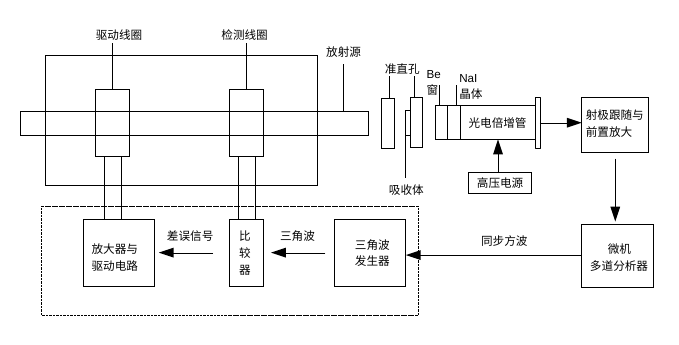
\includegraphics[width=\textwidth]{device.jpg}
    \caption{实验装置图}
    \label{fig:1}
\end{figure}
其中主要部件及作用解释如下:
\begin{enumerate}
    \item 放射源:本实验采用的是以$\rm{Pd}$(钯)为衬底的$^{57}\rm{Co}$放射源.为了使源发射的穆斯堡尔谱线是单色的,通常选用非磁性且具有立方晶系结构的金属做衬底.此外,所选金属也应具有较高的德拜温度以提高无反冲系数$f$.此外,选用金属做衬底的另一好处是,由于金属中电子的弛豫时间极短,前级衰变产生的局域电荷态将很快消失不起作用.
    \item 电磁驱动器:本实验采用的是背靠背双扬声器结构,其中分别含有一个驱动线圈和一个拾波线圈.驱动线圈用以达成周期性调制穆斯堡尔源所放出的$\gamma$射线的能量,拾波线圈则用来监测驱动线圈产生的信号.
    \item 驱动电源:来自多道分析器的同步方波经积分电路后变成三角波输入比较器.比较器将它与拾波线圈两端的信号相比较,其差值经放大器放大后再加于驱动线圈.实验中通常用示波器观察差误信号的大小,以监视驱动杆的运动是否正常.
    \item $\gamma$射线探测器:本实验使用的探测器是$\rm{NaI(Tl)}$闪烁体探测器.
    \item 微机多道分析器:在通用微机内插上线性放大卡、模数转换卡和多道分析卡就构成一台微机多道分析器.有脉冲幅度分析(PHA)和多度定标(MCS)两种功能.为了去除除$\si{14.4 keV}$的$\gamma$射线的影响,需要调节上下阈电位器.

\end{enumerate}
\subsection{实验操作内容安排}
\subsubsection{上下阈值的确定}
在不放置吸收体时,利用多道分析器的幅度分析工作方式测量实验所用的$^{57}\rm{Co}$放射源的$\gamma$能谱,并辨认出$\si{\num{14.4}keV}$的峰.然后合理设定上下阈值以滤除其他谱线.
\subsubsection{采集穆斯堡尔谱}
取多道分析器道数为512道,道时间间隔由电磁驱动器的固有周期(约0.1s)计算.正确设定多道分析器的参量后,开始采谱,并用示波器监视三角波信号或差误信号,必要时可调节驱动电源.分别测量$\alpha-\rm{Fe}$和硝普酸钠做吸收体时的穆斯堡尔谱.
\section{结果与分析}
实验采集的穆斯堡尔谱图分别如下:\par
\begin{figure}[htbp]
    \centering
    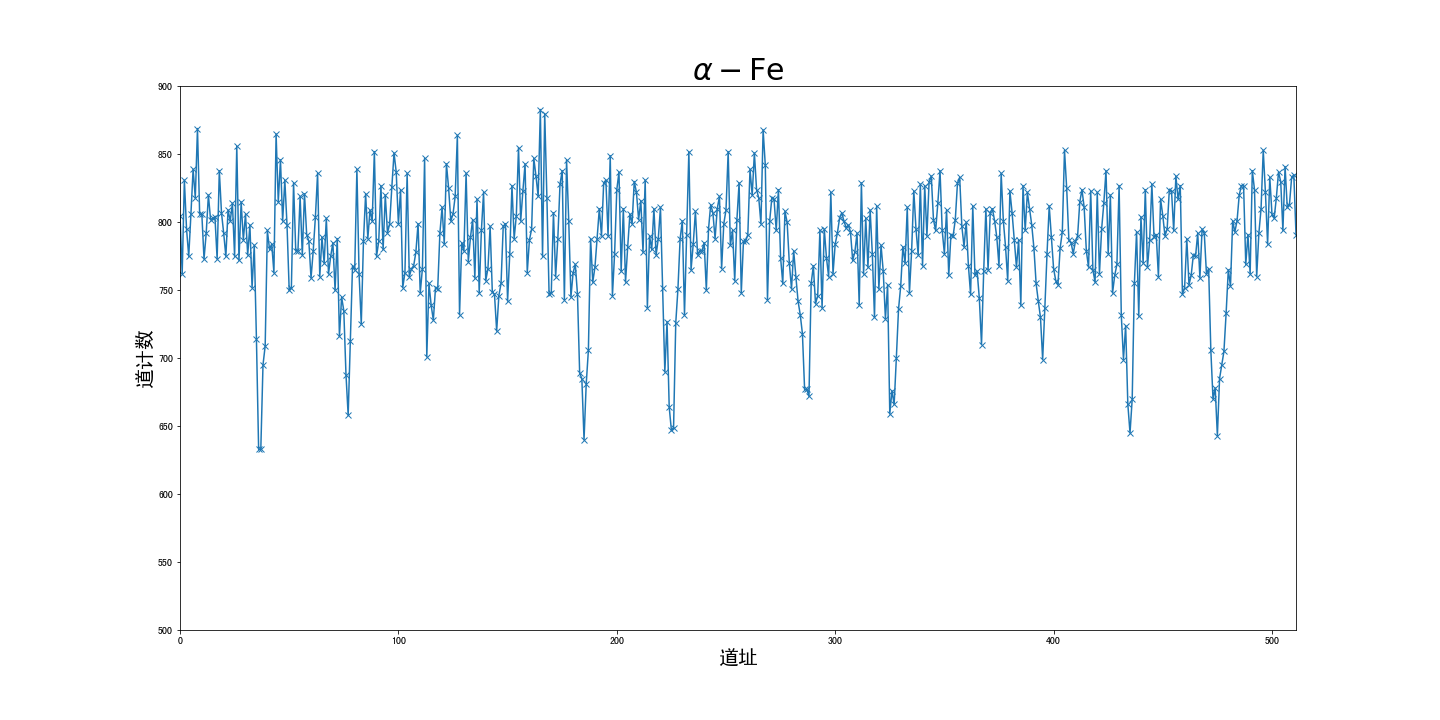
\includegraphics[width=\textwidth]{Exp_1/Fe.png}
    \caption{$\alpha-\rm{Fe}$的穆斯堡尔谱图}
    \label{fig:2}
\end{figure}
\begin{figure}[htbp]
    \centering
    \includegraphics[width=\textwidth]{Exp_1/NaX.png}
    \caption{$\rm{NaX}$的穆斯堡尔谱图}
    \label{fig:3}
\end{figure}
记录穆斯堡尔谱各峰位道址如下:\par
\begin{table}[htbp]
    \begin{ruledtabular}
    \centering
        \begin{tabular}{lrrrrrr}
            \toprule
            {$v_i$} &   1 &    2 &    3 &    4 &    5 ,&    6 \\
            \midrule
            道址1 &  37 &  77 &  113 &  145 &  185 &  225 \\
            道址2 &  475 &  435 &  395 &  367 &  325 &  288 \\
            \bottomrule
        \end{tabular}
    \end{ruledtabular}
    \caption{$\alpha-\rm{Fe}$的穆斯堡尔谱峰位}
\end{table}
\begin{table}[htbp]
    \begin{ruledtabular}
    \centering
        \begin{tabular}{lrrrr}
            \toprule
            {$v_i$} &    1 &    2 \\
            \midrule
            道址1 &  120 &  150 \\
            道址2 &  390 &  360 \\
            \bottomrule
        \end{tabular}
    \end{ruledtabular}
    其中,穆斯堡尔效应左右分别有一谱,且左侧从小到大,右侧从大到小。
    \caption{$\rm{NaX}$的穆斯堡尔谱峰位}
\end{table}
下根据穆斯堡尔谱图及数据进行分析:
\subsection{计算道增益$K$}
根据公式
$$K=\frac{10.656}{v_6-v_1}\si{mm\per s}$$
考虑由于存在批裂,采用如下式计算:
$$K=\frac{10.656*2}{|v^1_6-v^1_1|+|v^2_6-v^2_1|}\si{mm\per s}$$
得到道增益$K=0.056832\si{mm\per s}$.
\subsection{零速度对应道址}
首先分别确定两组谱线对应的重心位置,根据重心公式:
$$v_{c,\alpha-\rm{Fe}}=\frac{v_1+v_2+v_5+v_6}{4}$$
结合求出的道增益$K$,可得重心位置为
$$v^1_{c,\alpha-\rm{Fe}}=131;v^2_{c,\alpha-\rm{Fe}}=380.75$$
由于重心位置在$-0.185\si{mm\per s}$处,利用道增益可分别计算出零速度道址为:
$$v^1_{0}=134.25\si{mm\per s},v^2_0=377.49\si{mm\per s}$$

\section{结论}
首先要给出实验结果,然后再给出由实验结果分析得到的结果和结论.此部分给出的内容要比摘要中的全面,用词要更准确.\par

\section{致谢}
感谢王思广老师的悉心指导,也感谢和我一起参加实验的郜瑞啸同学,以及在同一实验室进行实验的赵萌同学.
%\bibliography{apssamp}
\begin{thebibliography}{}
\bibitem{Book} 吴思诚,荀坤 2015 近代物理实验(第四版)(北京:高等教育出版社)第80-91页.

\end{thebibliography}

\clearpage
\appendix
\section{思考题}
\subsection{问题一}
在发射(吸收)$\gamma$射线后,核的质量会有一定的下降(上升),带来的后果是,穆斯堡尔谱线会有一定的位移,但是由于多普勒效应的调节能量,加上$\gamma$射线引起的质量偏差很小,所以仍然可以看到穆斯堡尔谱.
\subsection{问题二}
当核赛曼分裂显著大于电四极裂距时,$^{57}\rm{Fe}$的能谱图应该接近于赛曼效应能谱图,而穆斯堡尔谱图也也接近,如下:
\begin{figure}[htbp]
    \centering
    \subfloat{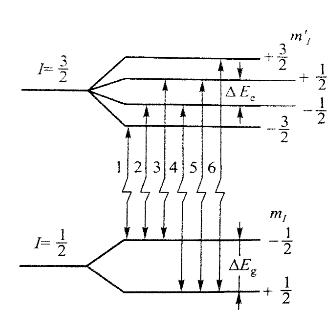
\includegraphics[width=0.3\textwidth]{zeeman.png}}....
    \subfloat{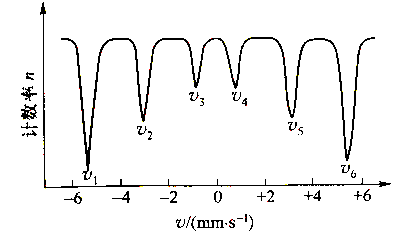
\includegraphics[width=0.3\textwidth]{zeeman_spe.png}}
    \caption{核赛曼分裂显著大于电四极裂距,左图为能谱,右图为穆斯堡尔谱}
    \label{fig:4}
\end{figure}
当核赛曼分裂显著小于电四极裂距时,$^{57}\rm{Fe}$的能谱图应该接近于电四极裂距能谱图,而穆斯堡尔谱图也也接近,如下:
\begin{figure}[htbp]
    \centering
    \subfloat{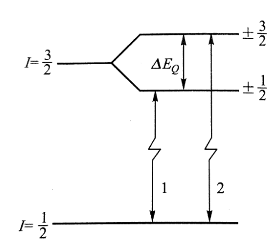
\includegraphics[width=0.3\textwidth]{quad.png}}....
    \subfloat{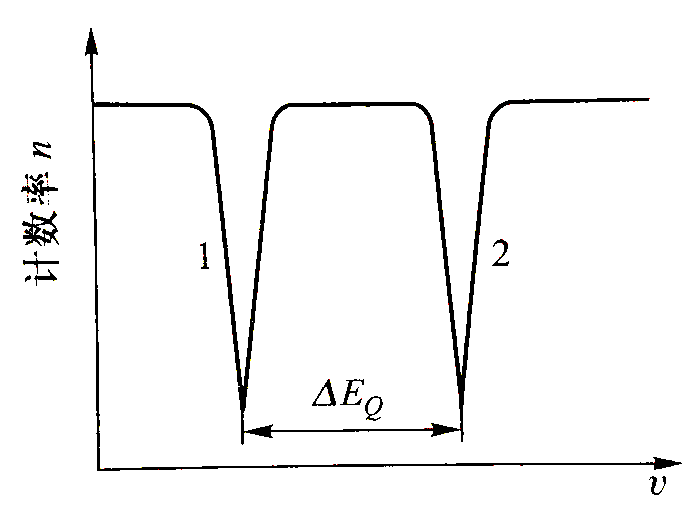
\includegraphics[width=0.3\textwidth]{quad_spe.png}}
    \caption{核赛曼分裂显著小于电四极裂距,左图为能谱,右图为穆斯堡尔谱}
    \label{fig:5}
\end{figure}
\subsection{问题三}
在源和吸收体较厚时,$\gamma$射线被吸收的可能性增大,使得吸收谱相应变宽.
\subsection{问题四}
考虑到$v_3$和$v_4$相隔较近,而峰值较小,误差较大,故不采用.
\end{document}